% Chapter Template

\chapter{Medical Modeling} % Main chapter title

\label{Chapter3} % Change X to a consecutive number; for referencing this chapter elsewhere, use \ref{ChapterX}
 
 %----------------------------------------------------

Digital modeling and rapid prototyping arise from the engineering need to quickly and cost-effectively design prototypes modeled using CAD software.\\
This request has led to an evolution of the software and equipment necessary to put this workflow into practice. Rapid prototyping has proved to be a useful tool, allowing to quickly evaluate the physical prototype and improve its digital design according to what it is found on the prototype, until a product that meets the required needs is obtained, iteration after iteration. \\
It was then realized that the same concept could be applied to other types of three-dimensional data, leading to the development of software to interface medical scans with rapid prototyping equipment. From the appreciation of the potential of this approach has developed the multidisciplinary field of Medical Modeling, which brings together engineers, radiologists, surgeons, designers, computer scientists and various other professionals, with the aim of using the acquired data from the patients to provide them with the highest standards of therapy \parencite{Reference1}.

\section{What can be done with patient images?}
Diagnostic images are extremely useful, both in everyday clinical practice and in research.
The digitization of acquisitions, the widespread use of computers and the variety of software available for data processing have allowed doctors to integrate imaging diagnostics into their daily activities. Diagnostic instruments are often sold by manufacturers with packages that include dedicated workstations and software. This should ensure, to the professional who buys the package, the full compatibility and integration of the dataflow between the purchased instruments. \\ 
When using medical imaging equipment, we do not work directly with the DICOM standard, but we are dealing with the implementation of the DICOM made by the manufacturer of the instrument used. This means that compatibility is not guaranteed, but we must rely on the \emph{DICOM Conformance Statement} that the manufacturer must attach to the tool, which indicates which functions of the DICOM standard have been implemented \parencite{Reference25}. \\
Proprietary software is certainly efficient, easy to use and often has good performance, especially when used on workstations marketed by the same manufacturer. At the same time these software are often not available outside of the packages comprehensive of the diagnostic equipment, or have a high cost to be purchased by institutions on a budget or by clinicians and students who want to approach the field. In addition, the fact that software is delivered with commercial license means that its source code is not accessible, and researchers working in the field have no way of developing new functions or testing new techniques on these software. \\
For these reasons, several open-source software have been developed, which allow researchers to use the general functions of medical image processing, such as DICOM file management and image visualization, and integrate functions for advanced images analysis and processing. \\
These software cover a large part of the workflow that we are going to analyze, and they provide other functionality that can be very useful when is required to perform advanced operations or create functions tailored to specific use cases.

\section{The digital model}
A three-dimensional model is a collection of points, connected to form lines, curves, polygons and volumes. Models can be created with appropriate modeling software, or acquired from the real world by means of scanning devices. \\
The act of creating a model, modeling, can be separate in \emph{organic modeling} and \emph{geometrical modeling}.

\begin{wrapfigure}{R}{0.35\textwidth}
% \ Centering
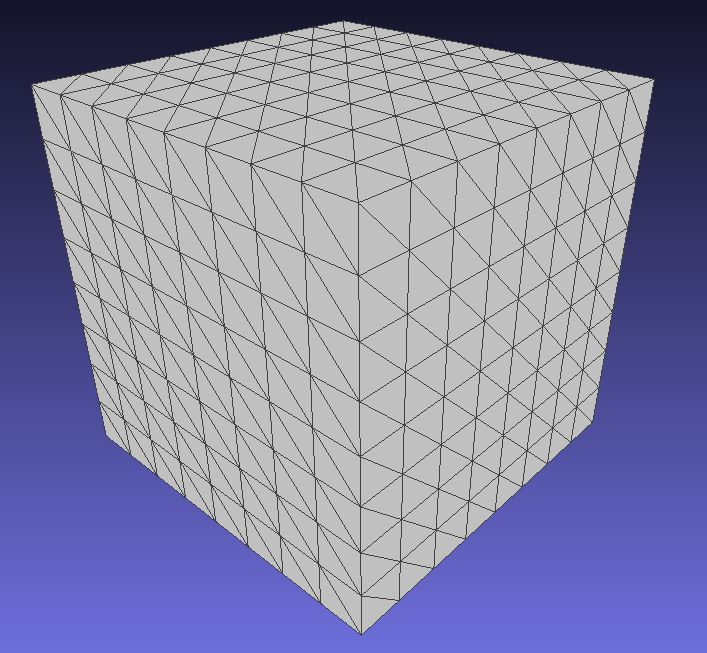
\includegraphics[width=0.35\textwidth, height=\textheight, keepaspectratio]{hr_cube_orga}
    \caption{cube made with organic modeling; a high number of mesh increases the resolution but complicates the modification of the volume shape.}
    \label{fig: hr_cube_orga}
\end{wrapfigure}

\paragraph{Organic modeling} is used to create natural geometries with rounded or irregular shapes, such as animals, plants, stones, humans and organs. The model consists of a surface made of polygonal faces, generally triangles, called \emph{mesh}. The density of polygons on the surface accounts for the resolution in the representation of details. Most of the models used in the medical field belong to this category, especially the models of parts of the human body. \\
The most common format for store organic models is the \textbf{.STL} (\emph{Stereolithography}, Standard Tasselation Language), which is a collection of triangular surfaces defined by the position of vertices in space and from the normals to the surfaces. The language was developed by 3D Systems for specific use with stereolithography machines, but it is now the standard language for models to be used with 3D printing. \\ A consortium of companies operating in the field of three-dimensional modeling and in additive manufacturing is currently at work for the creation of a new standard format, the \textbf{.3MF} (\emph{3D Manufacturing Format}) \parencite{Reference143}.

\begin{wrapfigure}{R}{0.35\textwidth}
% \ Centering
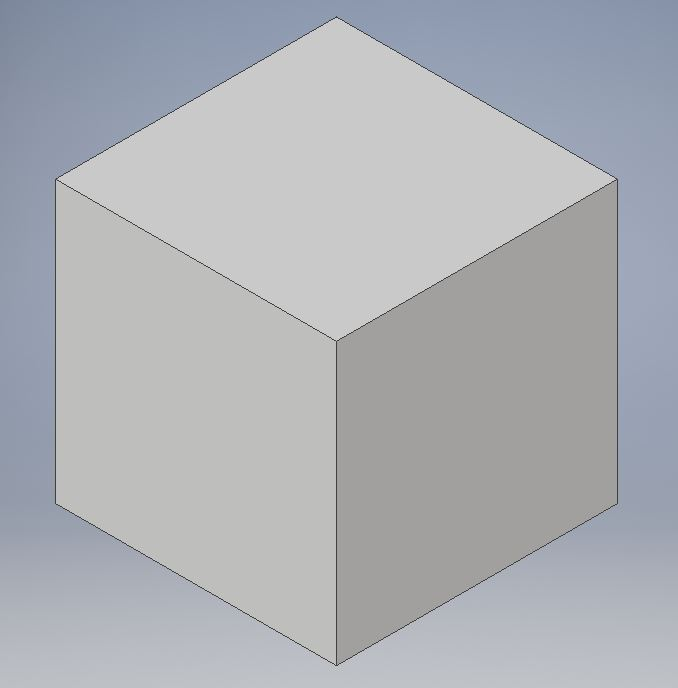
\includegraphics[width=0.35\textwidth, height=\textheight, keepaspectratio]{cube_geom}
    \caption {cube made with geometric modeling; the lowest number of faces is used to describe the cube.}
    \label {fig: cube_geom}
\end{wrapfigure}

\paragraph{Geometrical modeling} is used for the design of artificial parts, where the number of faces of the model must be optimized to simplify the design, the production and ensure the future adaptability of the design. The most widespread type of geometrical modeling is the \emph{parametric modeling}, adopted by major CAD software. Parametric modeling is based on the use of \emph{geometric primitives} (lines, curves \ldots) whose dimensions are defined and correlated. Parametric modeling is indicated for the design of engineering products, prosthesis and surgical guides. The output format of the model is dependent on the software used, but most parametric design software allows to export the models in .stl for the 3D printing procedures. The exported .stl model should be assessed for eventual conversion errors.

\section{3D Slicer}
3D Slicer is an open source software for the management and visualization of diagnostic images, made by developers and researchers in the medical field in a project supported by the \emph{National Institute of Health} (NIH), with the collaboration of companies such as \emph{Kitware Inc.} and \emph{General Electric}, and an expanding community of developers \parencite{Reference28}. \\
3D Slicer allows to manage DICOM files from \textbf{PACS} server (\emph{Picture Archiving and Communication System}) and non-specific archives, and allows to view and process images in 2D, 3D and 4D (X, Y, Z and T, \emph{time}, for example detection with ultrasound probes). The software offers the ability to render images and to create templates for use with CAD software \parencite{Reference31}.\\

From a software point of view, Slicer has a modular structure, with basic modules (\emph{Core modules}) that provide generic DICOM file management (\emph{DICOM}), rendering (\emph{Volume Rendering}) and the functions of image transformation in 3D space (\emph{Transforms}). Some of the other relevant modules are:
\begin{itemize}
\item \emph{\textbf{Filtering}}: contains tools for preparing the image for subsequent processing (\emph{preprocessing}). The most used features include arithmetic operations, noise reduction and correction of the density distribution of the scan, however there are dozens of other algorithms that can be used.
\item \emph{\textbf{Registration}}: provides the ability to align two scans with each other, useful when aligning different scans of the same patient, or orienting scans to standardize a dataset.
\item \emph{\textbf{Segmentation}}: segmentation is the separation of the image into smaller regions based on their characteristics. 3D Slicer integrates both interactive (with human input) and automatic segmentation methods.
\item \emph{\textbf{Surface models}}: allows the creation and management of surface volumes to be exported for further processing in other software.
\item \emph{\textbf{Image guided Therapy}}: gives the possibility to exchange data in real time with peripherals including robotic devices, scanners and radiotherapy devices.
This feature allows peripheral devices to be used in conjunction with diagnostic images, and may be of interest for use as \emph{virtual guide to implant placement} \parencite{Reference118}.
\end{itemize}

Other modules are present, and the collection is frequently expanded with modules created by the community, institutions and companies. Furthermore, each user can create a module and distribute it as a source or as a binary file (an executable file); this path can be used for packages that contain non-free proprietary code, but whose authors still want to distribute the functionality to the community \parencite{Reference28}. \\
The software is accompanied by publications and a documentation describing the implemented functionality \parencite{Reference28}, \parencite{Reference29}, \parencite{Reference30}. The documentation is the best reference for users who want to use the software and should be consulted to fully understand the operations performed by each module. There is also a forum on which is possible to communicate with 3d Slicer users and developers \parencite{Reference35}.

\section{Blender}
Blender \parencite{Reference32} is free and open-source software for computer graphics, maintained by the \emph{Blender Foundation} and a community of volunteer developers. It provides basic mesh creation and management, and advanced features such as animations, rendering and physical simulations. \\
Blender is a software that covers many aspects of computer graphics. It is accompanied by an extensive documentation of its features \parencite{Reference33}. The Blender community is important and has contributed to the maintenance of the software during its evolution, together with the Blender Foundation. The community is the place where to exchange ideas with experts and software users, where to find tutorials and workflow examples for all the features of Blender \parencite{Reference34}. \\
Blender is very useful for the post-processing of the models created in 3d Slicer. The software allows to modify the meshes of the model and to perform operations such as \emph{smoothing}, the modification of the size and resolution of the mesh and to use Boolean operations between two models (\emph{difference}, \emph{union} and \emph{intersection}). It also allows rendering to create high-quality images of the models.

\section{MeshLab}
MeshLab \parencite{Reference36} is free and open source software that allows advanced mesh processing, developed by students and researchers of the \emph{Faculty of Computer Science of the University of Pisa}. The software allows the import/export of a large number of format in which the models can be found and integrates tools for the inspection of the mesh and for its cleaning, algorithms for remeshing and creation of meshes from point clouds (optical scans, photogrammetry ...) and the management of the associated textures. \\
This software is useful for cleaning models, correcting problems with meshes, reducing the number of meshes and changing the shape and distribution of meshes on the model and comparing the models with each other.

\section{MeshMixer}
MeshMixer \parencite{Reference38} is not an open-source software, but it is a free software released by the company \emph{Autodesk}, which allows the visualization and processing of the meshes. MeshMixer is a software with many features, in some cases overlapping with software such as Blender and MeshLab, provided with a rich documentation \parencite{Reference39}. \\
This software provides an easy-to-use interface and excellent model manipulation and 3d printing preparation capabilities. MeshMixer simplifies the process of inspection and repair of the model, integrate analysis algorithms and tools for mesh processing. MeshMixer is a versatile tool that can be used in various step of the digital workflow. \\
When working with simple models, MeshMixer can speed up the preparation for printing, with tools that allow to perform Boolean operations, drill holes and repair defect of the mesh. The software facilitates the selection of areas of the model to be separated or in which to perform specific operations.

\section{FreeCAD}
FreeCAD \parencite{Reference40} is free and open-source parametric modeling software supported by a community of volunteer developers. The software allows to manage the production chain of an object. Integrate modules to perform the technical sketch and realize the 3D design from the sketch or by writing mathematical functions. Features modules for multi-part assembly and physical simulation, as well as various other applications such as robotics or boat design. \\
FreeCAD is useful for the realization of precise models, such as surgical guides and prostheses, but also parts created specifically for the 3D printer and allow to create objects of general utility such as supports and containers. It is a versatile software and a tool to known for anyone approaching 3D printing with the intention of creating functional and not merely aesthetic objects.\\
FreeCAD is supported by a frequently updated online documentation \parencite{Reference41}, and an ebook useful for understanding the basic functionality of the software, with practical examples aimed also at the 3D printing processing \parencite{Reference42}.

\section{Inventor}
Inventor \parencite{Reference43} is a professional CAD software developed by \emph{Autodesk}. It is among the most advanced parametric modeling software, and integrates all the functions of FreeCAD plus many others. The software is provided by Autodesk with a subscription plan, but for the students it is possible to download a 3-year trial version, very useful to have an approach with the software and to test its characteristics in depth. Inventor offers an easy approach to topology optimization via a dedicated module.

\section{nTopology Element}
nTopology \parencite{Reference139} is a commercial software for managing \emph{lattices} and \emph{scaffold}. It is a paid software but there is a free version that allows you to have an overview of the functions. The software facilitates the integration of 3D models and their conversion to scaffold.\\ It is possible to load physical simulations into nTopology, through which scaffolds can be obtained that will be optimized with respect to the loads that they will have to sustain. We will use the Free version of this scaffold generation software.

\section{Cura}
Cura \parencite{Reference44} is an open-source software for converting 3D models to g-code (slicing). The software is distributed by Ultimaker, a manufacturer of FDM 3D printers, and supported by a community of volunteer developers. Cura is supported by a documentation of the features \parencite{Reference45} and in-depth articles \parencite{Reference52}. \\
The software allows to perform slicing of the model and to adjust the printing options. Cura allows the adjustment of many parameters, including the printing temperature, layers height, filling geometry and its percentage. It also allows the automatic creation of various types of supports, and integrates the ability to work with more than one extruder in the same print, to make prints with more than one material.\\
Slicing is an important process in the printing workflow because it translates the digital model into a series of instructions. These are provided to the printer and result in a sequence of operations that it performs to give rise to a physical model, which aims to be the exact copy of the digital model.\\
Cura documentation describes the various printing parameters very well, so the main parameters will be briefly described here and the practical implications will be analyzed.

\subsection{Quality}
The \emph{\textbf{Quality}} menu contains parameters for adjusting the layer height and the width of the extruded line. Reducing the value of these items results in an increase in quality, because smaller details can be reconstructed. The choice of these parameters is not arbitrary, but is based on the characteristics of the printer.\\
The \emph{layer height} depends on the resolution of the extruder movement on the Z axis, which in turn depends on the steps/mm, based on movement mechanics and step interpolation (microstep). For example, a screw transmission with 8mm pitch, 1.8 degree/step stepper and 16x microstep, does a maximum 0.04mm step on the Z axis, which translates into a maximum resolution of 0.04mm on the Z axis, with the layer height to be set in multiples of 0.04 to have the maximum precision that this hardware is capable of. \\
Lower layer height allows you to reproduce smaller details and have a surface finish with a smoother appearance, but also increases the printing time, because you will need more layers to reproduce the model.\\
Setting the height of the first layer (\emph{Initial layer height}) with a higher value than the subsequent layers generally gives a better adhesion of the object to the print bed, because a more abundant flow of material in the first layer helps to compensate for a printing plane that is not perfectly horizontal. \\
The \emph{layer width} depends on the diameter of the \emph{nozzle} used, with smaller nozzles that increase the details reproduction, and large nozzles that reduce printing times; these are currently found in diameters ranging from 0.15 mm to over 1 mm. The layer width setting should be set to a value close to that of the nozzle diameters, maintaining a range of freedom to optimize the printing result. Setting a value slightly lower than the actual diameter can increase the print quality, but must be evaluated from time to time; moreover, a smaller width increases the printing time, because more lines will be used to make up the model. The value can be increased to compensate for any nozzle wear, but it is a temporary remedy and it is preferable to replace the worn nozzle with a new one.

\subsection{Shell}
The \emph{\textbf{Shell}} menu allows you to adjust the parameters of the model walls (shell). We can independently adjust the thickness of the model surfaces, roof and floor. A greater thickness will give a greater resistance to the model and a greater resistance to fluids leakage (\emph{leaking}) that can flow inside the model (\emph{microfluidic platform}). There are also various parameters regarding compensation for the expansion or shrinking of the print material and for fine-tuning the reproduction of the model surface.

\subsection{Infill}
The \emph{\textbf{infill}} is the filling of the model, the one that is inside the shell whose parameters we have explained before. The quantity of infill can be set in percentage, with 0\% indicating the absence of infill and 100\% indicating the complete filling of the volume of the object. There are several \emph{pattern} of infill, some fast as \emph{Lines} or \emph{Grid}, others slower but with better absorption of forces, such as \emph{Cubic subdivision}, while still others useful for printing deformable objects, such as \emph{Concentric} and \emph{Cross}. \\
The infill gives resistance to the object and acts as a support for the upper layers of the model. The percentage of infill must be adjusted according to the mechanical conditions in which the infill has to operate. A model that undergoes stress during use must have a high infill and a suitable geometry, while an aesthetic model can be made with little or no infill, in order to save material and speed up printing.\\
The infill menu contains several parameters that can be adjusted, among them the possibility to manually set the angle of some patterns (\emph{Infill Line Direction}). Manual adjustment of the infill line angle is a quick method in which the design of simple three-dimensional scaffolds can be performed \parencite{Reference138}.

\begin{figure}[h]
    \centering
    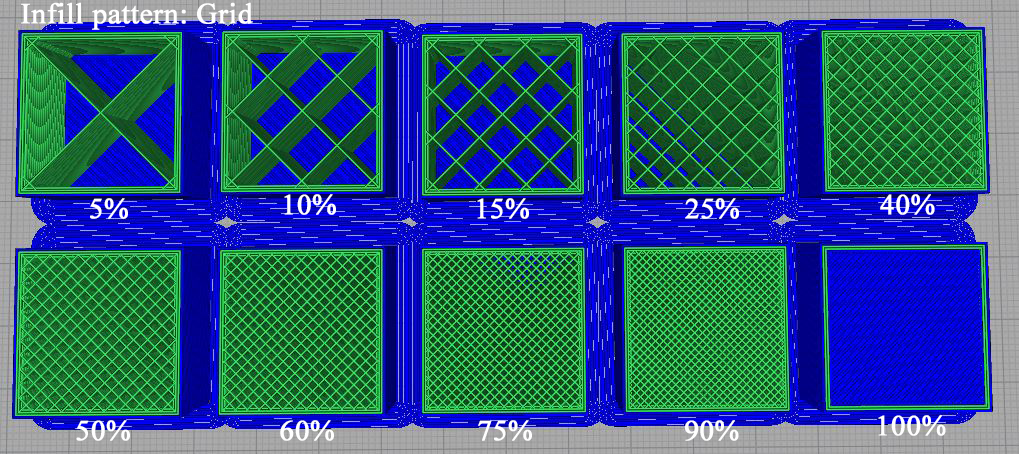
\includegraphics[width=\textwidth,height=\textheight,keepaspectratio]{numbers_grid_infillDens}
    \caption{\emph{\textbf{Infill pattern}}: \emph{Grid}; from left to right, progressive \emph{\textbf{Infill density}}.}
    \label{fig:numbers_grid_infillDens}
\end{figure}
	

\subsection{Material}
The \emph{\textbf{Material}} menu contains parameters for adjusting the temperatures and the extrusion process.
It is possible to adjust the \emph{printing temperature} and the temperature of the heated printing plate (\emph{build plate temperature}); you can set the temperature of the first layer independently of that of the subsequent layers. A higher temperature at the first layer favors the adhesion to the bed, because the extruded material is less viscous and flows better on the surface. The heated plate also facilitates adhesion, which is however related to the material of which the plate is made.\\
The \emph{flow} is regulated as a percentage and must be adjusted to avoid excesses or deficiencies of extruded material during printing. An adjustment method consists of observing the surface of the printed object to see if there are spaces or excesses between the layers, and varying the percentage of flow until it appears uniform. Another method is to print a cube without a roof, infill 0\% and with thick walls line (in \emph{shell} -> \emph{wall line count} = 1), and with a caliper measure whether the wall is actually thick the same value set in \emph{shell} -> \emph{wall line width}.
This empirical method can give an indication of the discrepancy between the actual width value and the real value. However, the relationship between the wall thickness and the flow value is not linear, because the extrusion quantity is influenced by parameters such as printing speed, actual filament diameter and printing temperature.\\
An important parameter is \emph{retraction}. Retraction is the distance that the filament is pulled back from the extruder each time a printed segment ends; this movement serves to reduce the pressure inside the nozzle and to limit the release of molten material during travels (\emph{oozing}). The values of retraction distance and retraction speed must be adjusted with appropriate tests, together with extrusion temperature and \emph{jerk}.

\subsection{Speed}
\begin{wrapfigure}{R}{0.4\textwidth}
\vspace{-20pt}
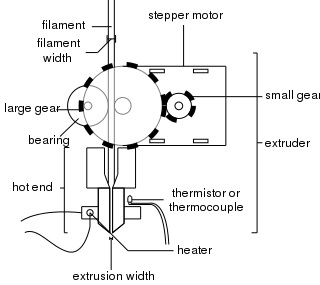
\includegraphics[width=0.4\textwidth, height=\textheight, keepaspectratio]{estrusore_diag}
    \caption{Direct extruder}
    \label{fig: estrusore_diag}
\end{wrapfigure}

The \emph{\textbf{Speed}} menu allows you to set the print speed. You can adjust the print speed of the shell and infill separately, the speed of travels and the accelerations during the various printing phases.
The \emph{jerk} is a parameter that manages the maximum instantaneous velocity change of the extruder; a low value smooths accelerations and decelerations while a high value makes them brusque. The effect of jerk is more evident when working at high speeds \parencite{Reference53}. \\
The printing speed must be adjusted according to the possibilities of the printer. Fast prints are generally less precise than slow prints, and for objects where accuracy is required a lower speed should be preferred. Fast prints cause vibration of the structure and instability in the flow of material, for which test prints must be made to evaluate how the printer behaves at various speeds.

\begin{wrapfigure} {R} {0.4\textwidth}
	%\centering
	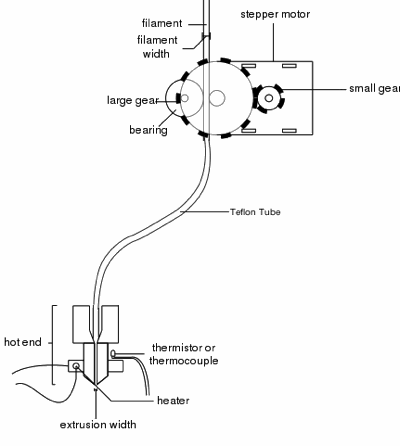
\includegraphics[width=0.4\textwidth, height=\textheight,keepaspectratio]{bowden}
    \caption{Bowden extruder}
    \label{fig:bowden}
\end{wrapfigure}

The speed also depends on the inertia of moving parts, so having a few light moving parts would help to increase speed in printing operations.\\
The filament extrusion system in FDM printers essentially consists of an extruder and an hotend. The extruder is the part that pushes the filament into the hotend, which warms up and melt the filament, which exit from the nozzle under the thrust of the extruder. On Cartesian FDM printers \emph{direct} extrusion is often used, which consists of the extruder connected to the hotend, both moving together on the axes.\\
To lighten the moving mass, and hence the inertia, it is possible to use an extrusion configuration called \emph{bowden} \parencite{Reference54}, \parencite{Reference55}, where the extruder is far from the hotend. The decrease in the moving mass, due to the dissociation between the extrusion process and the material melting process, allows printing at higher speeds without an excessive degradation of the printing quality. In the bowden extrusion the filament goes from the extruder to the hotend usually passing through a \emph{Teflon} (PTFE) tube, needing an obviously longer path than the direct extrusion; this makes the filament less responsive in the extrusion and retraction steps. This effect can be compensated for by adjusting the parameters of priming and retraction of the filament.

\subsection{Travel}
The \emph{\textbf{Travel}} menu contains options for managing printer movements during movements without extrusion. The \emph{Combing Mode} option restricts the movement of the nozzle to the print area of the model to reduce the need for retraction. This parameter can always be active, only active in the infill or off. To be adjusted according to the model to be printed, but pay attention to the fact that the nozzle moves on an already printed area and could damage it. Combing usually reduce printing time.
The \emph{Z-Hop} is a movement of the extruder on the Z axis at each retraction; by raising the extruder at the defined distance, it prevents the nozzle from touching the print during movements.

\subsection{Cooling}
The \emph{\textbf{Cooling}} menu provides tools for adjusting fan behavior during printing. During first layer printing the blower turned off favors good adhesion between the object and the printing plate; subsequently the fan speed can be increased up to 100\%. A good cooling of the material allows to print geometry with greater angles, using less supports for suspended areas (bridges). \\ Gradually increase the fan speed is preferable for the initial few layers, because it limits the deformation and detachment from the plane, especially with large prints. Some materials, such as \emph{nylon}, often require little or no cooling during printing, to prevent \emph{shrinkage} deformation.

\subsection{Support}
The menu \emph{\textbf{Support}} gives the possibility to create supports for the suspended or strongly inclined areas of the model. Various parameters can be adjusted on the quantity and shape of the supports, as well as the distance to be maintained by the object. During the creation of supports, a compromise must be sought between proximity to the object to be supported and ease in supports removal.

\begin{figure}[h]
	\centering
	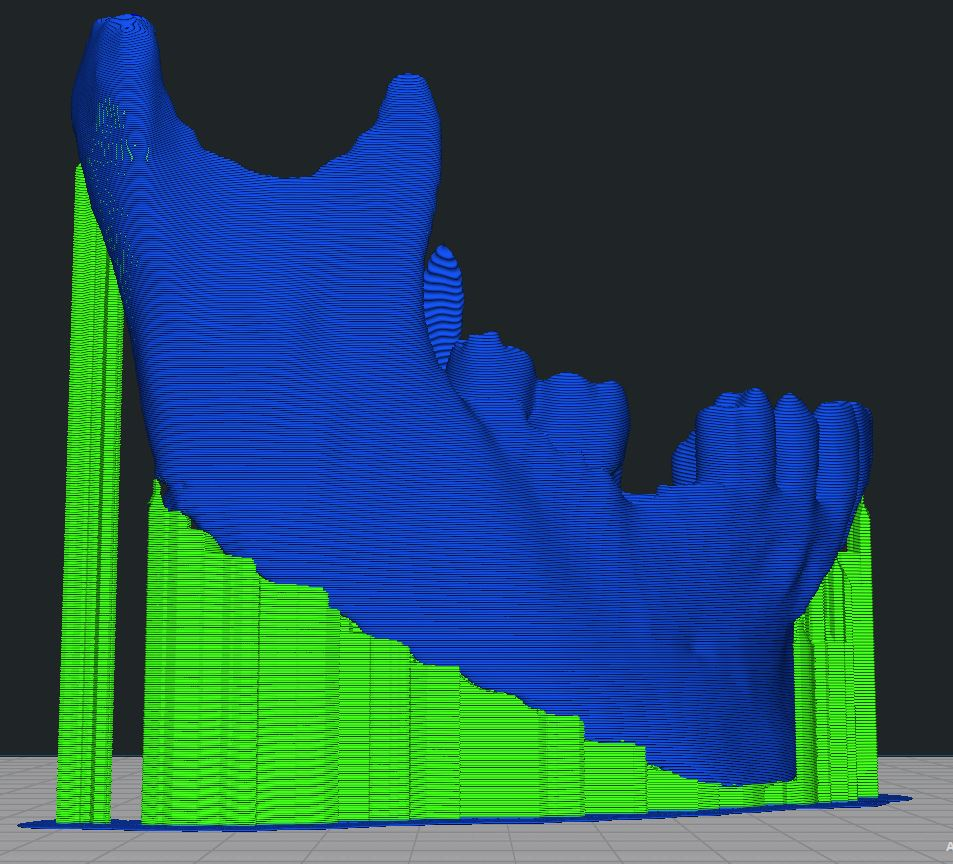
\includegraphics[width=0.5\textwidth, height=\textheight,keepaspectratio]{Supports}
    \caption{Supports in green}
    \label{fig:Supports}
\end{figure}

\newpage
	
\subsection{Build Plate Adhesion}
The \emph{\textbf{Build Plate Adhesion}} menu allows to generate contours or surfaces to facilitate the adhesion of the first layer to the plane.

\textbf{Skirt} is simply an extrusion turn made around the perimeter of the model to be printed, without touching it; it serves to prime the extruder, to extrude the material before printing so that the nozzle is ready to start the first layer.

\textbf{Brim} is a contour that joins to the edge of the first layer of the object. Its width can be adjusted and is an important help to keep the models sticking to the floor. It is also easy to remove and leaves virtually no marks on the model.

\textbf{Raft} is a few layers thick grid, produced between the printing plate and the object. Raft improves the adhesion even on an irregular surface and allows a good distribution of heat to the model. Useful for printing materials that deform greatly due to the printing process.

\begin{figure}[h]

\begin{subfigure}{0.3\textwidth}
\centering
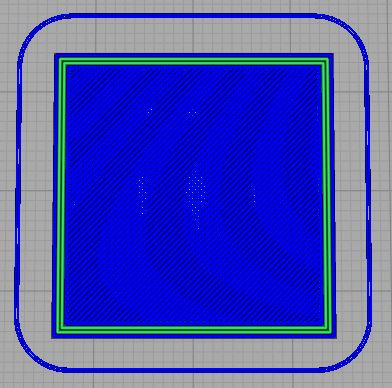
\includegraphics[width=0.6\linewidth, keepaspectratio]{skirt} 
\caption{Skirt}
\label{fig:skirt}
\end{subfigure}
\begin{subfigure}{0.3\textwidth}
\centering
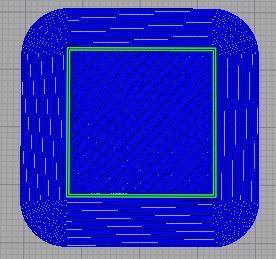
\includegraphics[width=0.6\linewidth, keepaspectratio]{brim}
\caption{Brim}
\label{fig:brim}
\end{subfigure}
\begin{subfigure}{0.3\textwidth}
\centering
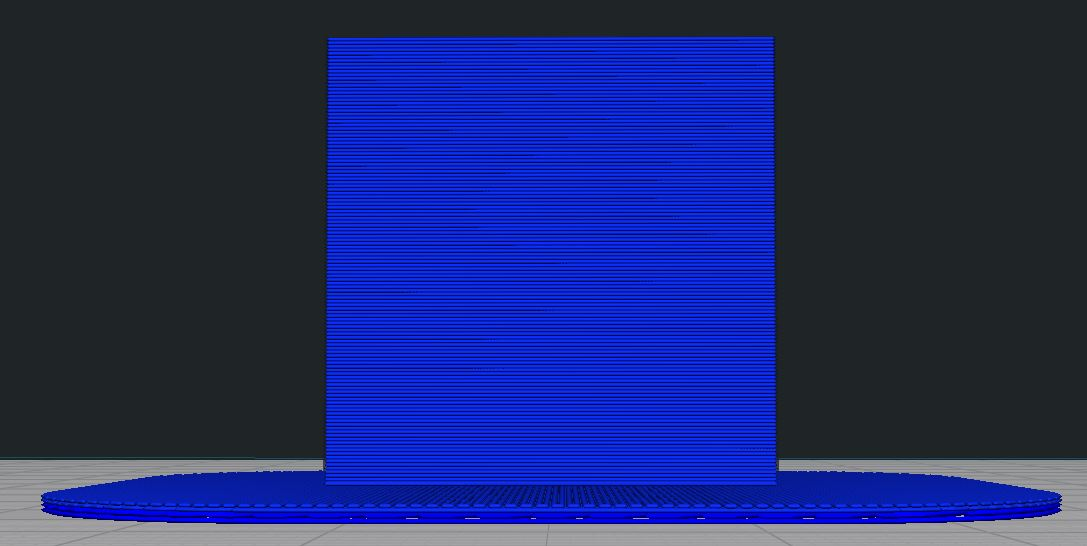
\includegraphics[width=0.8\linewidth, keepaspectratio]{raft}
\caption{Raft}
\label{fig:raft}
\end{subfigure}

\caption{\emph{Build Plate Adesion}.}
\label{fig:Build Plate Adesion}
\end{figure}
\vspace{-10pt}



\subsection{Fixes, Special Modes ed Experimental}
The other menus contain other advanced controls on the repair of the mesh during printing, special printing modes and experimental functions, which are not essential for the procedures here described, but which are still worth knowing, because they are useful in some situations.
In the \emph{\textbf{Special Modes}} we find the \emph{Print Sequence} option that gives the possibility to print objects on the plane all together or one at a time. \\
The \emph{Mold} option gives the possibility to create model negatives (a mold), which can be printed and used to recreate the original model by molding. \\
In \emph{\textbf{Experimental}}, the entry \emph{slicing tolerance} indicates how to slice the diagonal surfaces and affects the slicing mode \parencite{Reference56}. It is important to manage the tolerance of mechanical components that need adequate precision.
